\chapter{Tranzystor grafenowy}

Jak to działo się wiele razy w historii pojedyncze odkrycie, rzeczy z pozoru błahej daje początek
nowej idei, która staje się nowym kołem zamachowym dalszego rozwoju. Być może znajdujemy się 
w przededniu takiego odkrycia, porównywalnego do wynalezienia tranzystora. Mowa tutaj o grafenie, 
który jest bardo poważnym kandydatem na materiał w erze elektroniki post-krzemowej. 
Jako dowód tego stwierdzenia wystarczy wspomnieć, że grafen znajduje się na liście 
,,Międzynarodowej mapie technologii półprzewodnikowej" \footnote{The International Technology Roadmap for Semiconductors http://www.itrs.net/
Links/2009ITRS/Home2009.htm (Semiconductor Industry Association, 2009).}

Dzięki wzmożonej pracy wielu zespołów naukowych badających grafen. Już dzisiaj można mówić o realnej 
możliwości zastosowania tego materiału w procesie produkcji urządzeń elektronicznych. Mimo tak szybkiego 
rozwoju tej tematyki nie można w sposób jednoznaczny rozstrzygnąć panującej dyskusji, czy jest to na 
pewno wykonalne. 

W niniejszym rozdziale zostanie przedstawiona idea działania tranzystora FET. Prawdopodobnie najlepszej 
koncepcji urządzenia elektronicznego w dzisiejszym świecie. Następnie zostanie przedstawiona koncepcja 
zastosowania grafenu przy produkcji tego typu urządzenia. Wraz z omówieniem podstaw fizycznych jego działania,
modelami teoretycznymi, zostaną również przedstawione najważniejsze parametry z punktu widzenia inżynierii
stosowania takich urządzeń. Modele teoretyczne posłużą w następnym rozdziale do ich konfrontacji z danymi
eksperymentalnymi. Co zostanie opisane w następnym rozdziale. Na koniec zostanie przedstawiony proces 
wytwarzania takiego tranzystora.


	\section{Tranzystor FET}
Nazwa tego typu urządzenia pochodzi od angielskiego \textit{Field Effect Transistor}. Ze względu na największe
podobieństwo konstrukcji tranzystorów grafenowych do tranzystorów polowych typu MOSFET (\textit{ Metal-Oxide-Semi
conductur FET}), stanie się on podstawowym punktem odniesienia.
Budowa takiego urządzenie została przedstawiona na rysunku \ref{fig:MOSFET}. 


	\begin{figure}[ht]
	\centering
	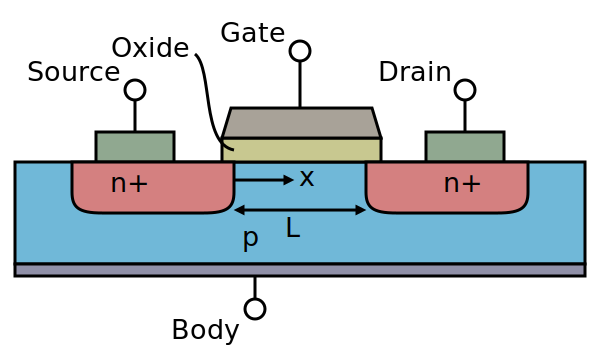
\includegraphics[width=0.50\textwidth]{./Rozdzial_3/obrazki/Lateral_mosfet}
	\caption{Przekrój ukazujący wewnętrzna budowę tranzystora typu MOSFET}
	\label{fig:MOSFET}
	\end{figure}

Jak widzimy na podłożu typu p zostały wytworzone obszary typu n, stanowiące źródło i dren. Zazwyczaj obszary te 
powstają na drodze implantacji jonów lub dyfuzji atomów domieszek do podłoża. Pomiędzy tymi obszarami w efekcie 
zjawiska polowego powstaje kanał. Kanał tworzy  się, gdy pomiędzy bramkę a podłoże zostanie przyłożone napięcie. 
Dla tranzystora typu n-kanałowego, napięcie musi być dodatnie. Po przyłożeniu dodatniego napięcia, elektrony 
z podłoża zaczynają gromadzić się pod bramką. W ten sposób jako nośniki mniejszościowe sprawiają, że obszar ten
staje się obszarem wyróżnionym pod względem zwiększenia jego przewodności. Dzięki temu przy przyłożonym napięciu 
pomiędzy drenem a źródłem zaczyna płynąć prąd. 

Taki tranzystor może znajdować się w 3 obszarach pracy. Wyłączony, brak wytworzonego kanału, duża oporność pomiędzy
drenem i źródłem. Obszar liniowej pracy kiedy to prąd drenu zależy w przybliżeniu liniowo od napięcia dren-źródło. 
Wreszcie obszar nasycenia, gdzie prąd źródło-dren słabo zależy od zmian napięcia pomiędzy nimi. Wszystkie te sytuacje
przedstawia rysunek \ref{fig:MOSFET_char}.


	\begin{figure}[ht]
	\centering
	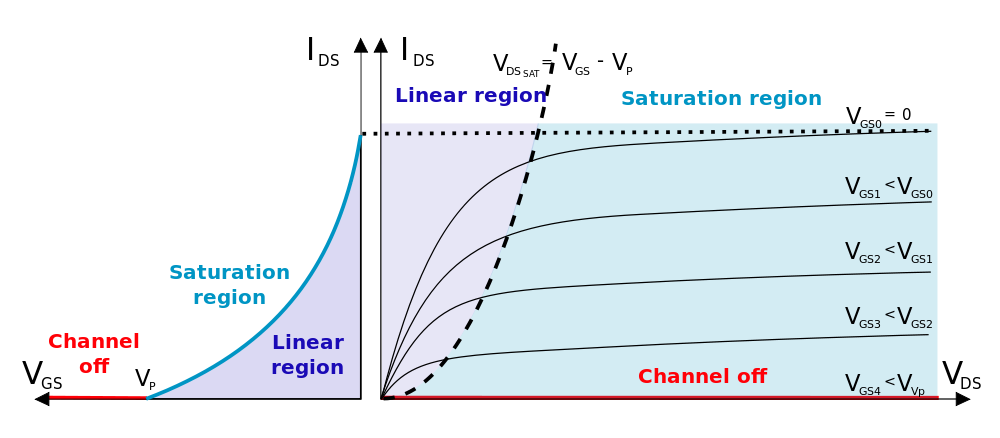
\includegraphics[width=0.90\textwidth]{./Rozdzial_3/obrazki/Charakterystyki_FET}
	\caption{Zależność prądu płynącego przez tranzystor}
	\label{fig:MOSFET_char}
	\end{figure}

Matematycznie można to opisać równaniem:

\begin{equation}
    \mathrm{ I_{DS}(V_G, V_{DS}) = \mu C_{ox} \frac{W}{L}[(V_G - V_T)V_{DS} - \frac{V_{DS}^2}{2}]}
	\label{equ:prad_drenu}
\end{equation}

Wyróżniamy dwa podstawowe typy charakterystyk elektrycznych tranzystorów FET. Pierwszym jest charakterystyka przejściowa,
którą otrzymuje się gdy prąd drenu otrzymuje się jako funkcję napięcia bramkowego, przy stałym napięciu źródło-dren. 
Drugim typem jest tak zwana charakterystyka wyjściowa będąca funkcją prądu drenu do napięcia dren-źródło, przy stałym 
napięciu bramkowym.

Mierząc te charakterystyki i porównując je ze wzorem \ref{equ:prad_drenu}, można wyznaczyć ruchliwość badanego tranzystora, $\mu$. 
Znając inne parametry występujące we wzorze, gdzie: L-długość kanału, W-szerokość kanału, 
$\mathrm {C_{ox}}$-powierzchniowa gęstość
 pojemności pomiędzy kanałem a bramką, $\mathrm{ V_G}$-napięcie bramkowe,
 $\mathrm{ V_{DS}}$-napięcie dren-źródło, $\mathrm{ V_T}$-tak zwane napięcie progowe.
Pomiary tych charakterystyk stały się podstawą do wyciągnięcia wniosków o właściwościach transportowych grafenu, użytego
w roli kanału.

Dzisiaj w świecie inżynierii elektronicznej istnieją dwie podstawowe grupy określające zastosowanie danego tranzystora. 
Zastosowania w układach logicznych lub w układach radiowych. W zasadzie można powiedzieć, że albo do zastosowań cyfrowych
albo do zastosowań analogowych. 

Relatywnie większą łatwość wprowadzania nowych technologicznie materiałów obserwuje się w segmencie analogowym. Wynika, to
głównie z tego względu, że wydajność urządzeń cyfrowych najbardziej zależy od najgorszych egzemplarzy tranzystorów 
zintegrowanych w układzie logicznym. Podczas, gdy w przypadku pojedynczo produkowanych tranzystorów do zastosowań analogowych,
te z nich, które za bardzo odbiegają parametrami od norm mogą zostać niedopuszczone do sprzedaży. Co odbywa się bez wpływu
dla reszty sprzedawanych egzemplarzy tranzystorów. To samo tyczy się zintegrowanych układów scalonych. Jako znacznie
prostsze są mniej narażone na ewentualne odchyłki parametrów pojedynczego tranzystora.

Jednak pomimo różnic, obie te gałęzie dążą do wspólnych celów. Zmniejszenia kosztów produkcji pojedynczego tranzystora.
Polepszenia jego właściwości. Głównie dla tranzystorów przeznaczonych do zastosowań cyfrowych działaniem mającym na celu
 zaspokojenie obu tych wymagań przez wiele lat było sukcesywne zmniejszanie pojedynczego tranzystora. Dzięki temu stawały
 się one szybsze. Zajmując mniej miejsca na podłożu oszczędzały drogi krzem.

Dzięki tym zabiegom złożoność układów cyfrowych mogła się podwajać co 18 miesięcy. Ta zależność jest nazywana ,,prawem
Moora". Jednocześnie takie układy stawały się tańsze.

Ze zmniejszaniem się pojedynczego tranzystora rosły wymagania co do procesu technologicznego, w którym je produkowano.
Dzisiejsze fabryki układów scalonych stały się niesłychanie kosztownymi przedsięwzięciami (kosztującymi miliardy dolarów).
Właśnie te linie produkcyjne są jednym z powodów całkowitego opanowania przez krzem technologii produkcji układów
 cyfrowych, ponieważ budowa nowej fabryki pochłonie więcej pieniędzy niż modernizacja obecnej. Należy pamiętać, że postępem
rządzi ekonomia.

To rozwiązanie zaczęło zawodzić, kiedy zaczęto dochodzić rozmiarami tranzystora do granic możliwości. Wtedy stało się jasne,
że niezbędne będzie opracowanie całkowicie nowej technologii wytwarzania lepszych tranzystorów.

Wspomniana technologia układów cyfrowych opiera się na komplementarnych tranzystorach CMOS (\textit{Complementary Metal-
Oxide-Semiconductur}). Podstawowym budulcem bramek logicznych jest para tranzystorów MOS z kanałami n i p. Oba mogą 
znajdować w dwóch stanach: włączenia i wyłączenia. Najwięcej energii pobierane jest, gdy chcemy zmienić ten stan. 
Idea polega na takim projektowaniu układów logicznych by poszczególne bramki logiczne składały się z kombinacji
tranzystorów n i p kanałowych, która zapewnia brak przepływu dużych prądów w stanie ustalonym. Często najbardziej znaczącym
prądem w stanie ustalonym jest suma prądów upływności bramek. Są one niezbędne do poprawnej polaryzacji bramki.
Z tego powodu bardzo pożądaną właściwością tych tranzystorów jest duży stosunek prądu włączenia do prądu wyłączenia, z 
warunkiem minimalizacji prądu wyłączenia. Typowymi wartościami są tutaj stosunki wł/wył wynoszące 10$^4$--10$^7$
\footnote{gr. tranz. ref 2}.  W typowych konstrukcjach poszczególnych FET-ów wymaga to posiadania wystarczająco szerokiej
przerwy energetycznej najlepiej więcej niż 0,4 eV. Drugą ważną właściwością jest posiadanie dokładnie takiego samego
napięcia przełączania. Dopiero te dwa warunki są w stanie zapewnić dobrego kandydata na następce dla dzisiaj stosowanych
materiałów.


Sytuacja w dziedzinie zastosowań analogowych, ze szczególnym wskazaniem zastosowań radiowych, wygląda z goła inaczej. 
Tutaj sama miniaturyzacja tranzystora nie jest najważniejsza, bo ważniejsze są jego właściwości, a same zintegrowane układy
analogowe są znacznie bardziej proste niż cyfrowe. Dodatkowo badania nad wieloma technologiami były i są wspierane przez
 agencje wojskowe. Dzięki temu produkty wysokiej jakości, ale będące drogie znajdują swoje zastosowania. Dzięki temu ten
 segment rynku jest znacznie bardziej otwarty na nowe technologie. Jako przykłady można wspomnieć tutaj np o tranzystorach
HEMT, opartych na materiałach III-IV; urządzeniach opartych na technologii arsenku galu GaAs, lub fosforku indu InP.


W zastosowaniach analogowych nie wymaga się od tranzystora posiadania stanu całkowitego wyłączenia. Zazwyczaj i tak 
w większości zastosowań tranzystory te pracują w jakimś punkcie pracy, który wymusza stały przepływ prądu. Tutaj dużo 
ważniejszym parametrem jest z kolei liniowość i wysoka częstotliwość odcięcia. W przypadku grafenu co zostanie pokazane
poniżej warunek liniowości jest bardzo dobrze spełniony. Tak samo jak spełniony jest ten o wysokiej częstotliwości odcięcia.
Donosi się o tranzystorach grafenowych o specjalnej budowie, gdzie rolę bramki pełni nanoprzewód, dla których
częstotliwość odcięcia zawierała się w przedziale 100--300 GHz \footnote{High-speed graphene transistors with a self-aligned nanowire gate}.



Podsumowując, z powodów tutaj przedstawionych wynika, że technologia grafenu ma większą szansę zaistnieć 
w wysokoczęstotliwościowych zastosowaniach analogowych. Dodatkowe argumenty potwierdzające tą tezę znajdują się 
w kolejnej części, mówiącej o czysto fizycznych aspektach stosowania grafenu do produkcji urządzeń elektronicznych.

	\section{Tranzystor FET z kanałem grafenowym}
		\subsection{Podstawy fizyczne działania}


	
	W szerokich paskach grafenowych może istnieć wile pojedynczych kanałów przewodnictwa. Transport przez te kanały
	jest proporcjonalnie zmniejszany względem długości całego paska. Szerokość natomiast ma wpływ na wzrost liczby
	dostępnych kanałów. Zakładając, że mówimy tutaj o sytuacji, w której znajdujemy się w pobliżu punktów Diraca.
	Można napisać, że:

	\begin{equation}
    		\mathrm{ G \sim \frac{e^2}{h}\frac{W}{L} }
		\label{equ:G}
	\end{equation}
	Gdzie W-szerokość paska grafenowego, L-jego długość. Wzór \ref{equ:G}, pochodzi z \footnote{http://arxiv.org/abs/cond-mat/0603315}.
	Ta zależność prowadzi do wniosku, że przewodność skaluje się tutaj tak jak w przypadku funkcji przewodnictwa w 
	metalach dyfuzyjnych. 


		\begin{figure}[ht]
	\centering
	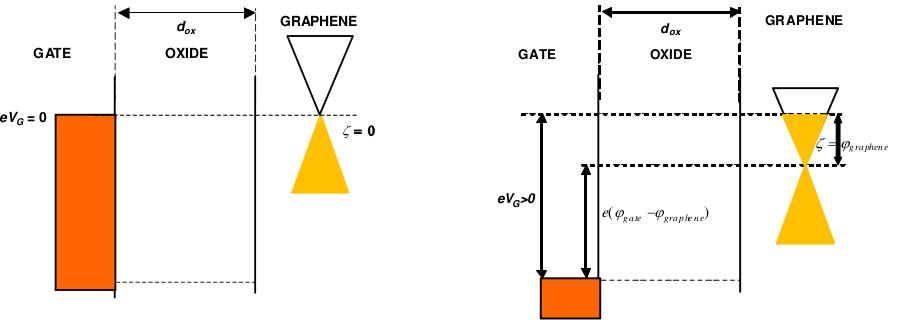
\includegraphics[width=0.90\textwidth]{./Rozdzial_3/obrazki/zasadadzialania.jpg}
	\caption{Zasada działania tranzystora grafenowego}
	\label{fig:MOSFET_dzialanie}
	\end{figure}

	
	Zależność koncentracji od napięcia bramkowego jest liniowa, a koncentracja wiąże się również liniowo z 
	przewodnictwem\footnote{http://jpsj.ipap.jp/link?JPSJ/71/1318/}. Co zostało zaprezentowane w poprzednim rozdziale.
	 Z tego wynika, że zależność przewodności jest liniową funkcją napięcia bramkowego co zostało pokazane empirycznie
	np. przez \footnote{http://www.ncbi.nlm.nih.gov/pmc/articles/PMC1180777/}.
	Jedynym miejscem, gdzie nie jest to prawdą jest okolica występowania minima przewodnictwa. Jest to związane, ze 
	zmianą typów nośników. 

	
	Tranzystory grafenowe mają bardzo interesujące i niespotykane charakterystyki przejściowe. Przykład takiej 
	charakterystyki znajduje się na rysunku \ref{fig:GFET_trans}. Typ nośników jak również ich koncentracja
	zależą od napięcia pomiędzy bramką a kanałem. Dla dużych napięć ujemnych obserwujemy akumulację dziur w kanale
	i w tym obszarze charakterystyka świadczy, o kanale typu p. Duże napięcia dodatnie na bramce prowadzą do akumulacji
	elektronów w kanale i dla tego obszaru charakterystyka wskazuje na kanał typu n.
	
	Taki mechanizm powoduje powstanie dwóch niezależnych obszarów w charakterystyce przejściowej, które rozdzielone są
	punktem minimalnego przewodnictwa, punktem Diraca. Położenie tego punktu na charakterystyce zależy od wielu 
	czynników. Po pierwsze od różnicy pracy wyjścia materiału bramki i grafenu, co można zobaczyć na obrazku 
	\ref{fig:MOSFET_dzialanie}, czyli od konstrukcji samego urządzenia. Bardzo ważnym czynnikiem jest również 
	wszelkie domieszkowanie kanału. Wpływ na domieszkowanie mają defekty strukturalne jak również wszelkie 
	zanieczyszczenia, powstałe w skutek ekspozycji na powietrze, lub domieszkowanie celowe. Innym ważnym czynnikiem 
	jest też koncentracja i typ ładunków na interfejsach dolnych, i górnych (np. dla urządzenia typu top-gate).
	


	Jak widać na rysunku \ref{fig:MOSFET_dzialanie}, zmieniając napięcie bramkowe zmieniamy położenie 
	poziomu Fermiego w kanale. Zmieniając ten poziom sterujemy gęstością stanów poszczególnych nośników 
	Dlatego zwiększając napięcie obserwujemy wzrost koncentracji elektronów w kanale i spadek koncentracji dziur.
	Wtedy kanał staje się typu n. Natomiast, gdy zmniejszamy napięcie bramkowe, obniżamy ten poziom a wraz z nim
	koncentrację elektronów i tym samym zwiększamy koncentrację dziur. Takie zachowanie wynika wprost ze struktury
	pasmowej grafenu, a zwłaszcza z obszaru styku pasm przewodnictwa i walencyjnego, tak zwanych stożków Diraca, 
	o których była mowa w poprzednim rozdziale. 

	Ważne jest by zauważyć iż gęstość stanów jest zależna w sposób liniowy od napięcia bramkowego, co znowu wynika
	ze struktury pasmowej tego materiału. Gęstość stanów ma bezpośredni wpływ na koncentrację, a od koncentracji
	w sposób również liniowy zależy przewodność kanału. Podsumowując napięcie bramkowe steruje w sposób liniowy
	przewodnością kanału. Dodatkowo polaryzacja napięcia ma wpływ na typ akumulowanego ładunku w kanale i tym samym
	na jego typ (n lub p).
	

		\subsection{Najważniejsze właściwości}
			\paragraph{Ruchliwość}
%\addcontentsline{toc}{subsection}{Ruchliwość} To jest teraz nie potrzebne już

	Jest to najczęściej podawana zaleta grafenu. Zwłaszcza zdolność do jej zachowania nawet w temperaturach 
	pokojowych, co zostało omówione w poprzednim rozdziale, wraz z podaniem jej wartości dla poszczególnych 
	przypadków grafenu na różnych podłożach.
	Wysokie wartości osiąganych ruchliwości w tym materiale robią duże nadzieje na znalezienie dla tego materiału
	odpowiedniego zastosowania. 
	
	Problemem jest tutaj to, że tak duże wartości są osiągane dla dużych próbek grafenu, które z kolei nie posiadają 
	przerwy energetycznej. Jest to znaczna wada, co zostało wykazane w poprzednim podpunkcie. 
			\paragraph{Przerwa energetyczna}


	Jak zostało wspomniane przerwa energetyczna jest bardo pożądaną własnością. Powody zostały przedstawione na początku
	tego rozdziału. Istnieją metody takiej inżynierii grafenu, zdolne wytworzyć przerwę energetyczną w grafenie. 
	Jednak skutkuje to bardzo znacznym zmniejszeniem ruchliwości, czyli głównej zalety tego materiału.
	Mówiąc bardziej ilościowo, dla metody stosowania tak zwanych nanowstążek grafenowych ruchliwości wynoszą około 
	200 $\mathrm{\frac{cm^2}{V s}}$, co jest wielkością o trzy rzędy większości mniejszą niż w grafenie pochodzącym
	z eksfoliacji, o dużo większej powierzchni. \footnote{tutaj odnośniki z 1 rozdziału}

Dlatego podsumowując najlepiej było by opracować taką technologię, która wymaga wysokiej ruchliwości i nie wymaga posiadania
przerwy energetycznej. Zamiast przystosowywać ten materiału do znanych nam obecnie technologii. Dlatego w dalszym ciągu
ewentualne zastosowania w przemyśle pozostają kwestią otwartą.

\paragraph{Dwuwymiarowość}
	Powołując się na teorię skalowania tranzystorów typu MOSFET\footnote{Robert Dennard 1974}, 
	dostatecznie cienki obszar kanału pozwoliłby 
	na skalowanie długości bramki do bardzo małych rozmiarów. Co z kolei zapewniłoby wzrost częstotliwości odcięcia
	i poprawiło parametry takiego tranzystora w porównaniu do innych. Dwuwymiarowa postać grafenu zapewnia najmniejszą
	grubość kanału jaka w ogóle jest możliwa do osiągnięcia. Dlatego wedle tej teorii tranzystory grafenowe powinny się
	łatwiej skalować od tych opartych na materiałach trójwymiarowych. Oczywiście należy zauważyć, iż ta teoria dotyczy 
	tylko półprzewodników, a grafen jest półmetalem i taki kanał nie posiada przerwy energetycznej. Jednak
	 nanowstążki wykazują taką przerwę zatem dla nich ta teoria powinna być prawdziwa. Jednak jak już wspomniano
	w przypadku nanowstążek obserwowane ruchliwości są znacznie mniejsze niż dla grafenu masywnego. Być może okaże się,
	że dzięki możliwości skalowania takich nanowstążkowych tranzystorów wzrośnie znacznie szybkość ich przełączania. 
	Co w połączeniu z możliwością ich wyłączenia stanie się podstawą do stosowania ich w układach logicznych, gdzie
	te właściwości są najbardziej decydujące, a ruchliwość ma znaczenie drugorzędne. 

		\subsection{Omówienie charakterystyk elektrycznych}

	\begin{figure}[ht]
	\centering
	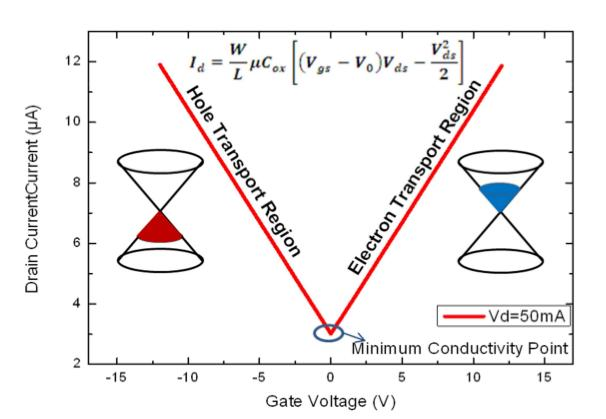
\includegraphics[width=0.90\textwidth]{./Rozdzial_3/obrazki/charakterystykaPrzej}
	\caption{Wygląd typowej charakterystyki przejściowej tranzystora GFET}
	\label{fig:GFET_trans} 
	\end{figure}

Pierwszą i mającą w zasadzie największe znaczenie dla wyznaczania najważniejszych parametrów charakteryzujących tranzystory 
jest charakterystyka przejściowa. Charakterystyka przejściowa zbierana jest, gdy mierzony jest prąd płynący przez kanał, 
przy stałym napięciu dren-źródło w funkcji napięcia bramkowego. Często prąd zamieniany jest na wielkość zapewniającą
bardziej obiektywny wgląd w faktyczne zmiany właściwości materiału jaką jest przewodność, ewentualnie rezystywność. 
Taka typowa charakterystyka została przedstawiona na obrazku \ref{fig:GFET_trans}. Jak widać, charakterystyka jest liniowo 
zależna od napięcia bramkowego, oprócz obszaru w okolicy minimum przewodnictwa. 


	\begin{figure}[ht]
	\centering
	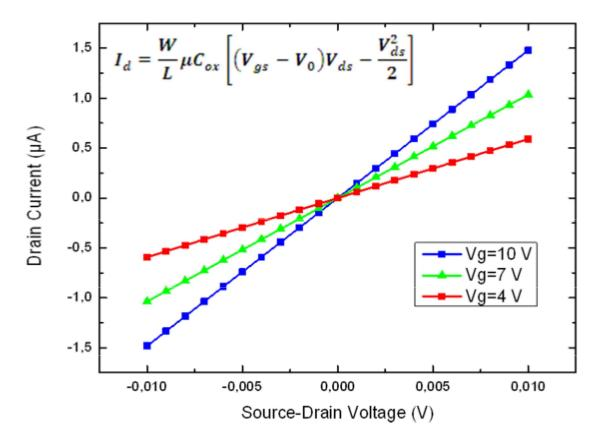
\includegraphics[width=0.90\textwidth]{./Rozdzial_3/obrazki/charakterystykaWyj.jpg}
	\caption{Wygląd typowej charakterystyki wyjściowej tranzystora GFET}
	\label{fig:GFET_out} 
	\end{figure}

Drugim typem charakterystyki jest charakterystyka wyjściowa. Pomiarów tej charakterystyki dokonuje się poprzez 
Ustawienie stałego napięcia bramkowego i wyznaczeniu prądu dren-źródło w funkcji napięcia dren-źródło. Typowy wygląd 
charakterystyki dla grafenu został przedstawiony na rysunku \ref{fig:GFET_out}. Tutaj również często zamienia się prąd na
przewodność lub rezystywność. Ten rodzaj charakterystyki zazwyczaj ma mniejsze znacznie dla charakteryzacji.

\subsection{Proponowane modele transportu}
W niniejszej pracy zaprezentowano kilka najczęściej proponowanych podjeść do wyznaczania parametrów transportowych urządzeń
grafenowych. Głównym parametrem wyznaczanym dla tych urządzeń jest ruchliwość. Istnieją co najmniej trzy metody jej 
wyznaczania. 
\paragraph{Model Drudego}

Pierwszym z modeli transportu jest model Drudego. Model Drudego zazwyczaj znajduje zastosowanie w opisie metali. Grafen 
jest półmetalem dlatego istnieją przesłanki do jego stosowania. Model ten opiera się na kinetycznej teorii gazów, gdzie
zamiast gazu mamy do czynienia z tak zwanym gazem elektronowym. Elektrony tak jak molekuły gazu poruszają się chaotycznie
zderzając się z jonami sieci krystalicznej. Po przyłożeniu pola elektrycznego powstaje kolektywny ruch w kierunku działania 
pola, który jest nałożony na te chaotyczne drgania termiczne. 
W ogólności można zapisać:

\begin{equation}
    \mathrm{ \vec J =q n_{ind} \mu_{Drude} \vec E }
\end{equation}

Z tego równania na gęstość prądu można po prostych przekształceniach otrzymać równanie używane do określenia ruchliwości 
dla próbek grafenowych:

\begin{equation}
   \mathrm{ \sigma = C_{ox}} V_G\mathrm{ \mu_{Drude}}
	\label{equ:przewodnoscDrudego}
\end{equation}

Gdzie C$_{ox}$-gęstość powierzchniowa pojemności, opisana wzorem:
\begin{equation}
   \mathrm{C_{ox}= \frac {\epsilon_o \epsilon_r}{d_{ox}}}
\end{equation}

Dzięki temu funkcja przewodności $\sigma$, zależy tylko od jednego parametru w sposób liniowy. To znaczy od napięcia
bramkowego $V_G$. Mając takie opis matematyczny i dysponując zmierzonymi charakterystykami przejściowymi, wyznaczenia
ruchliwości dokonuje się dopasowywyjąc zmierzoną przewodność do tej oczekiwanej. Parametrem dopasowywanym jest oczywiście
ruchliwość, ponieważ inne zmienne występujące w równaniu \ref{equ:przewodnoscDrudego}, są albo znane.

Dla tego modelu donosi się o wysokich ruchliwościach przy wysokiej koncentracji nośników. \footnote{1,17 model tr. gr.}

\paragraph{Model stałej ruchliwości}
Model zakładający stałą ruchliwość nośników w grafenie, niezależnej od koncentracji, zaproponowany został przez 
\footnote{S. Adam, E. H. Hwang, and S. Das Sarma, Physica E 40, 1022 (2008).}. 
Dzięki takim założeniom można zapisać wzór na opór elektryczny próbki jako :

\begin{equation}
    \mathrm{ R_{całkowite} = 2R_{kontakt}+ \frac{L}{W}\frac{1}{\mu \sqrt{e^2 n_o + C_{ox}^2(V_G-V_{Dirac}^2)}}}
	\label{equ:stalaRuch}
\end{equation}

W przypadku równania \ref{equ:stalaRuch} również dopasowywuje się to równanie do danych eksperymentalnych. Parametrami
dopasowania są w tym przypadku: R$_{kontatkt}$-będące opornością kontaktów, stałą ruchliwość $\mu$  i koncentrację nośników
n$_o$.

\paragraph{Model ruchliwości Halla}
Ta metoda wyznaczania ruchliwości jest również często stosowana, choć wymaga ona dodatkowego sprzętu laboratoryjnego. 
Przedstawiając w sposób najprostszy polega ona na wyznaczaniu zależności oporu przy stałych napięciach bramkowych
w obecności zmiennych pól magnetycznych. 

Ta metoda nie znalazła zastosowania w niniejszej pracy. Dlatego nie zostanie ona opisana dokładniej.

\paragraph{Metoda techniczna (to jest chyba do zmiany!)}
Istnieje jeszcze metoda wykorzystująca ogólny model tranzystora FET. Opisany równaniem \ref{equ:prad_drenu}, gdzie po 
prostych przekształceniach i założeniu, że znajdujemy się w liniowym obszarze charakterystyki przejsciowej, można napisać:

\begin{equation}
    \mathrm{ \mu_{FE} = \frac{L}{W}\frac{g_m}{C_{ox}V_{DS}}}
\end{equation}
\begin{equation}
    \mathrm{ g_m = \frac{d I_D}{d V_G} |_{ V_{DS}=const}}
\end{equation}

Ogromną zaletą tej metody jest jej uniwersalność i możliwość porównywania tranzystorów wykonanych nawet w zupełnie innej
technologii i przy użyciu innych materiałów. 

Nie jest ona niestety pozbawiona wad. Duży wpływ na wartość otrzymanej ruchliwości ma wybór części charakterystyki. 
Dlatego istnieje tutaj sporo miejsca do nadużyć, lub popełniania błędów. Jednak w przypadku urządzeń grafenowych, nie ma
to aż takiego znaczenia, ponieważ te charakterystyki są liniowe w szerokim zakresie. Dlatego również ta metoda jest dobra
do oszacowania ruchliwości.

	\section{Najnowsze technologie tranzystorów grafenowych}

	Typowe schematy budowy tranzystorów grafenowych zostały przedstawiona na rysuku \ref{fig:MOSFET_struktury}. 
	Widoczne są tutaj dwa najczęściej stosowane podłoża, to znaczy podłoże krzemowe i podłoże węglika krzemu.
	Jak widzimy najmniej skomplikowanym schematem jest pierwszy od lewej, czyli tak zwany bottom-gate. 
	Gdzie rolę bramki pełni podłoże krzemowe domieszkowane w odpowiedni sposób. Tranzystory tego typu 
	pojawiły się już na samym początku badania grafenu w roku 2004. Jednak ich zaleta, to znaczy prostota, znacznie
	ogranicza ich stosowanie w jakimś praktycznym zastosowaniu. Wystarczy tutaj tylko wspomnieć, że duża wielkość
	bramki i jej duża pojemność powodują, niską częstotliwość odcięcia. Niemniej taki typ budowy wciąż jest 
	stosowany w badaniach transportowych właśnie ze względu na swoją prostotę i to, że pozwala obserwować topografię
	grafenu np. przy pomocy mikroskopii AFM co jest niezbędne w niektórych badaniach.

	Drugim typem budowy jest top-gate, gdzie na kanale nałożony jest materiał dielektryczny, na którym została napylony
	elektryczny kontakt bramki. Taka budowa tranzystora jest znacznie bardziej zbliżona do dzisiaj stosowanych co 
	pozwala na łatwiejsze porównywanie takich tranzystorów z obecnie produkowanymi. Zwłaszcza w kwestii długości bramki
	w odniesieniu do częstotliwości odcięcia. Często pozostawia się dodatkowo dolną bramkę służącą porównaniu 
	osiągnięć dla każdej z nich, lub badaniu wpływowi dielektryka na własności transportowe. Tylnia bramka okazuje się
	być również niezwykle przydatna w czasie procesu produkcji.Pozwala stwierdzić, czy kontakty
	drenu i źródła są odpowiednio nałożone, czy tranzystor reaguje już na napięcie bramkowe.
	Problemem tego typu tranzystorów bywa wpływ nałożenia dielektryka na zmniejszenie się ruchliwości. Minimalizacja
	tego problemu jest wciąż obiektem badań.

	Ostatnim najczęściej spotykana koncepcja  tranzystora jest oparta o grafen otrzymany z węgliku krzemu. Ważne jest,
	że węglik krzemu w ogólności jest przewodzący, dlatego należy stosować jego wersję półprzewodzącą. Zwiększa to 
	koszt produkcji jednak pozwala w ogóle takim tranzystorom działać. Z tego też względu jedyną bramką jest bramka
	górna. Znowu ten rodzaj tranzystora jest podobny do obecnie wytwarzanych i w tym przypadku nie odbiega zbytnio swoją
	koncepcją od poprzedniego. Tutaj również istnieje problem pogorszenia parametrów kanału po nałożeniu dielektryka 
	bramkowego.

Największe nadzieje wiązane są ze strukturami top-gate. Przede wszystkim ze względu na większe możliwości miniaturyzacji i 
lepszej optymalizacji bramki. Co ma wpływ na szybkość tranzystora. Częstotliwość odcięcia wiąże się z długością bramki jak
L$^{-1}$, gdzie L jest długością bramki. Ruchliwość również wpływa na szybkość, zwiększając ją. Typowe MOSFET oparte na 
krzemie wykazują ruchliwości rzędu 100 $\mathrm{\frac{cm^{2}}{Vs}}$, struktury typu pHEMT oparte o arsenek galu 6 000
$\mathrm{\frac{cm^{2}}{Vs}}$, natomiast te oparte o fosforek indu 10 000 $\mathrm{\frac{cm^{2}}{Vs}}$
\footnote{Chodzi tutaj o tak zwane ruchliwości efektu polowego dla gotowych już urządzeń}.
Przy coraz mniejszych długościach bramki ruchliwość przestaje mieć duże znaczenie na szybkość tranzystora i większy wpływ
zaczynają mieć efekty związane z impedancjami pasożytniczymi i efekty krótkiego kanału. 
Co prawda tranzystory grafenowe są wciąż gorsze niż konwencjonalne tranzystory pracujące w wysokich częstotliwościach. To
jednak już wyprzedziły swoimi parametrami te oparte o krzem i powoli zbliżają się do struktur opartych o arsenek galu.
Donosi się o tranzystorze opartym na nanowstążce grafenu, pokrytej dielektrykiem HfO$_2$ (dielektryk o wysokiej stałej 
dielektrycznej), który w temperaturze pokojowej osiągnął stosunek prądów wł/wył wynoszącą 70 i niesamowitą transkonduktancję
wynoszącą 3,2 $\mathrm{mS}{\mu m}$ (co jest lepszym wynikiem niż najlepsze tranzystory krzemowe MOSFET i HEMT oparte na 
arsenku galu ). \footnote{ref 82 z tr. gr. review}
	

	\begin{figure}[ht]
	\centering
	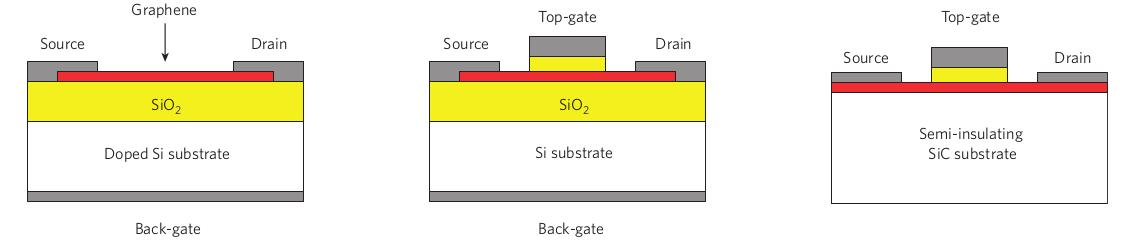
\includegraphics[width=1.00\textwidth]{./Rozdzial_3/obrazki/TypuBudowa}
	\caption{Spotykane struktury tranzystorów grafenowych}
	\label{fig:MOSFET_struktury}
	\end{figure}

	\section{Proces produkcji tranzystorów z kanałem grafenowym}

W tej części zostanie opisany proces otrzymywania tranzystorów z transferowanego grafenu CVD, na podłoże krzemowe, o
 strukturze bottom-gate. Ze względu na to, iż dokładny opis wszystkich etapów takiej produkcji byłby bardzo obszerny, 
zostanie on tutaj przedstawiony w lakonicznej formie. Będzie on dotyczył metodologii otrzymania tranzystorów, które
zostały poddane charakteryzacji, a jej wyniki posłużyły jako dane eksperymentalne dla poniższej pracy dyplomowej.

\subsection{Produkcja grefenu i transfer}
Ten etep w zasadzie został już opisany przy okazji opisu samej metody CVD. Z tego też względu należy w zasadzie tylko
dodać, że grubość SiO$_2$ wynosiła 300nm. Próbki zostały zakupione od firmy Graphenea. Próbki przed dalszymi
etapami produkcji zostały poddane charakteryzacji. Polegała ona na wykonaniu skanu topografii mikroskopem sił atomowym
i spektroskopii Ramana.



\begin{figure}[ht]
        \centering
        \begin{subfigure}[b]{0.48\textwidth}
                \centering
                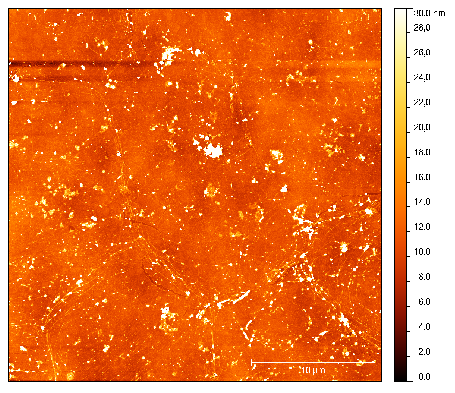
\includegraphics[width=\textwidth]{./Rozdzial_3/obrazki/AFMCVD}
                \caption{Mapa topografii AFM}
                \label{fig:AFMCVD}
        \end{subfigure}%
        ~ %add desired spacing between images, e. g. ~, \quad, \qquad etc.
          %(or a blank line to force the subfigure onto a new line)
        \begin{subfigure}[b]{0.48\textwidth}
                \centering
                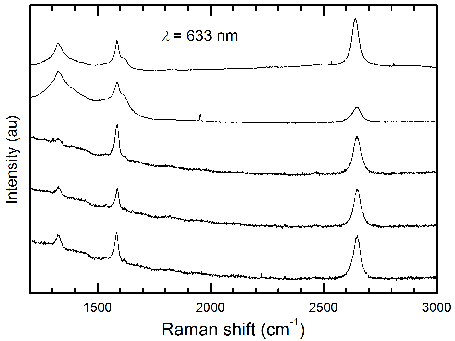
\includegraphics[width=\textwidth]{./Rozdzial_3/obrazki/RAMAN}
                \caption{Widma Ramanowskie grafenu}
                \label{fig:RamanCVD}
        \end{subfigure}
\end{figure}

Mapa topografii wskazuje na wysoką czystość próbki, jako, że wysokość na próbce waha się jedynie w granicach 0--30 nm.
Otrzymane widma Ramana wskazują na dobrą jakość strukturalną grafenu. Porównując je z wykresem pochodzącym z literatury
staje się jasne, że mamy do czynienia z jedną warstwą grafenową \footnote{Raman spectroscopy in graphene, 
Physics Reports, vol. 473, no. 5–6, pp. 51–87, Apr. 2009.}, rysunek \ref{fig:RamanCVDLiteratura}.

	\begin{figure}[ht]
	\centering
	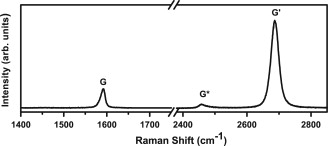
\includegraphics[width=.60\textwidth]{./Rozdzial_3/obrazki/RAMANodniesienie}
	\caption{Wykres przykładowego widma Ramana }
	\label{fig:RamanCVDLiteratura}
	\end{figure}
\subsection{Nałożenie kontaktów drenu i źródła}
	Kolejnym krokiem w procesie produkcji było nałożenie kontaktów elektrycznych dla drenu i źródła. W celu
optymalizacji struktury postanowiono wykorzystać jeden wspólny kontakt dla wszystkich tranzystorów, stanowiący źródło. 

Proces wytwarzania kontaktów rozpoczyna się od nałożenia przy pomocy spin-coatera rezystu. Następnie rezyst zostaje 
naświetlony przy pomocy wcześniej zaprojektowanej maski. W taki sposób by po wywołaniu wytworzyły się zagłębienia, 
stanowiące formy dla przyszłych elektrod. 
Następnym krokiem jest napylenie na całą powierzchnię próbki metalu, tworzącego elektrody. Do usunięcia zbędnych obszarów
z nałożonego metalu używa się metody lift-off. Polega ona na zanurzeniu próbki w rozpuszczalniku pozostałego rezystu i 
poddaniu próbki działania ultradźwięków.
Dzięki temu otrzymujemy pożądany wzór elektrod na powierzchni próbki.

Oczywiście nie jest to metoda idealna ze względu chociażby na wytworzenie się "uszu" na krawędziach elektrod. Jest to
o tyle niebezpieczne, że taka wysoka cienka krawędź może opaść i wytworzyć zwarcie, zwłaszcza, gdy elektrody znajdują 
się w bardzo bliskich odległościach. Innym często spotykanym problemem jest gdy mimo wypłukania rezystu spod warstwy 
metalu ten dalej się utrzymuje. Zazwyczaj kończy się to zniszczeniem próbki ze względu na niemożność usunięcia tego
nadmiaru metalu.

Największą zaletą tej metody jest to, że nie wykorzystuje ona żadnych agresywnych chemikaliów do trawienia. Ma to istotny
wpływ na utrzymanie jakości badanego grafenu.

\subsection{Wytwarzanie kanału}

W kolejnym kroku należy usunąć nadmiar grafenu, który teraz pokrywa przestrzeń pomiędzy wszystkimi elektrodami. 
Osiąga się to poprzez wykonanie nałożenie rezystu i wywołaniu go w taki sposób by wytworzył warstwę ochronną nad 
miejscami, w których pozostać ma grafen. 

Tak przygotowaną próbkę poddaje się trawieniu plazmowemu, otrzymując w zasadzie gotową już próbkę. Wystarczy teraz 
tylko usunąć resztki ochraniającego rezystu i próbka jest już gotowa.

	\begin{figure}[ht]
	\centering
	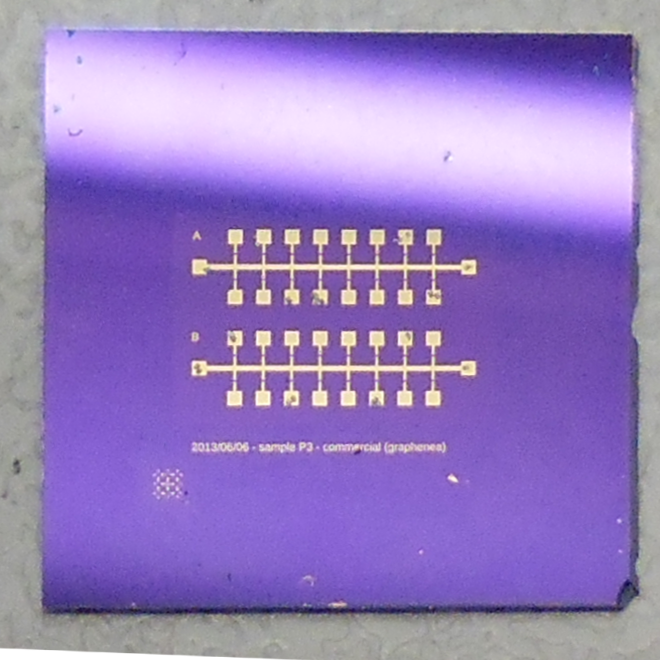
\includegraphics[width=.65\textwidth]{./Rozdzial_3/obrazki/Probka}
	\caption{Gotowa próbka}
	\label{fig:GotowaProbka}
	\end{figure}

Zdjęcie przedstawione na rysunku \ref{fig:GotowaProbka} przedstawia taką gotową strukturę. W lewym dolnym rogu
widoczne są markery niezbędna przy naświetlaniu kolejnych masek. Widoczna jest też topografia próbki. 
Jak widać wszystkie tranzystory zostały wytworzone wzdłuż jeden masywnej elektrody. Ta elektroda stanowi
umownie źródło. Dreny kolejnych tranzystorów są połączone ze źródłem poprzez kanały grafenowe. Przykładowy skan
takiego pojedynczego kanału przedstawiony został na obrazkach \ref{fig:AFMCVDkanal} i \ref{fig:AFMCVDkanalfaza}. 

\begin{figure}[ht]
        \centering
        \begin{subfigure}[b]{0.48\textwidth}
                \centering
                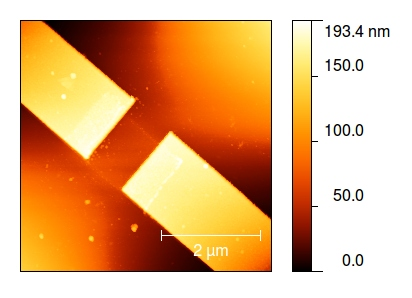
\includegraphics[width=\textwidth]{./Rozdzial_3/obrazki/20130521-g32}
                \caption{Topografii AFM jednego z kanałów}
                \label{fig:AFMCVDkanal}
        \end{subfigure}%
        ~ %add desired spacing between images, e. g. ~, \quad, \qquad etc.
          %(or a blank line to force the subfigure onto a new line)
        \begin{subfigure}[b]{0.48\textwidth}
                \centering
                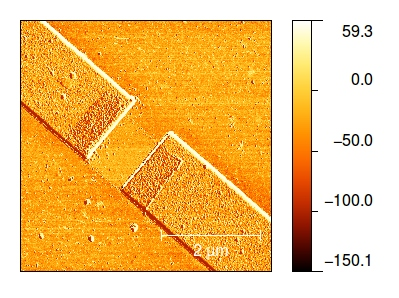
\includegraphics[width=\textwidth]{./Rozdzial_3/obrazki/20130521-g32faza}
                \caption{Skan fazowy AFM}
                \label{fig:AFMCVDkanalfaza}
        \end{subfigure}
\end{figure}

Pomiary AFM wykonane zostały w trybie kontaktu przerywanego. Dzięki temu możliwe było uzyskanie, oprócz
skanu topograficznego, skanu fazowego. Skan topograficzny dostarcza informacji bezpośrednio o wysokości na próbce.
Skan fazowy zapewnia informacje związaną z kontrastem materiałowym. Niestety ze względu na skomplikowaną naturę 
oddziaływań igły z danym materiałem dokładana analiza ilościowa jest bardzo utrudniona. Dlatego postanowiono
ograniczyć się do stwierdzenia, że na skanie widoczne są trzy materiały. Podłoże z SiO$_2$, złote elektrody i 
kanał grafenowy. Co więcej skany AFM pozwoliły określić realne wymiary kanałów badanych tranzystorów 
niezbędne do wyznaczania parametrów tranasportowych. Zostanie do dokładniej opisane w następnym rozdziale.

